\documentclass{article}

\usepackage{graphicx}
\usepackage{tikz}
\usepackage{tikzsymbols}
\usetikzlibrary{calc,patterns,shapes.geometric}
\pagestyle{empty}
\usepackage[margin=0pt]{geometry}
\geometry{papersize={14in,12in}}

\def\centerarc[#1](#2)(#3:#4:#5){\draw[#1] ($(#2)+({#5*cos(#3)},{#5*sin(#3)})$) arc (#3:#4:#5);}

\begin{document}
	\begin{figure}
		\centering
		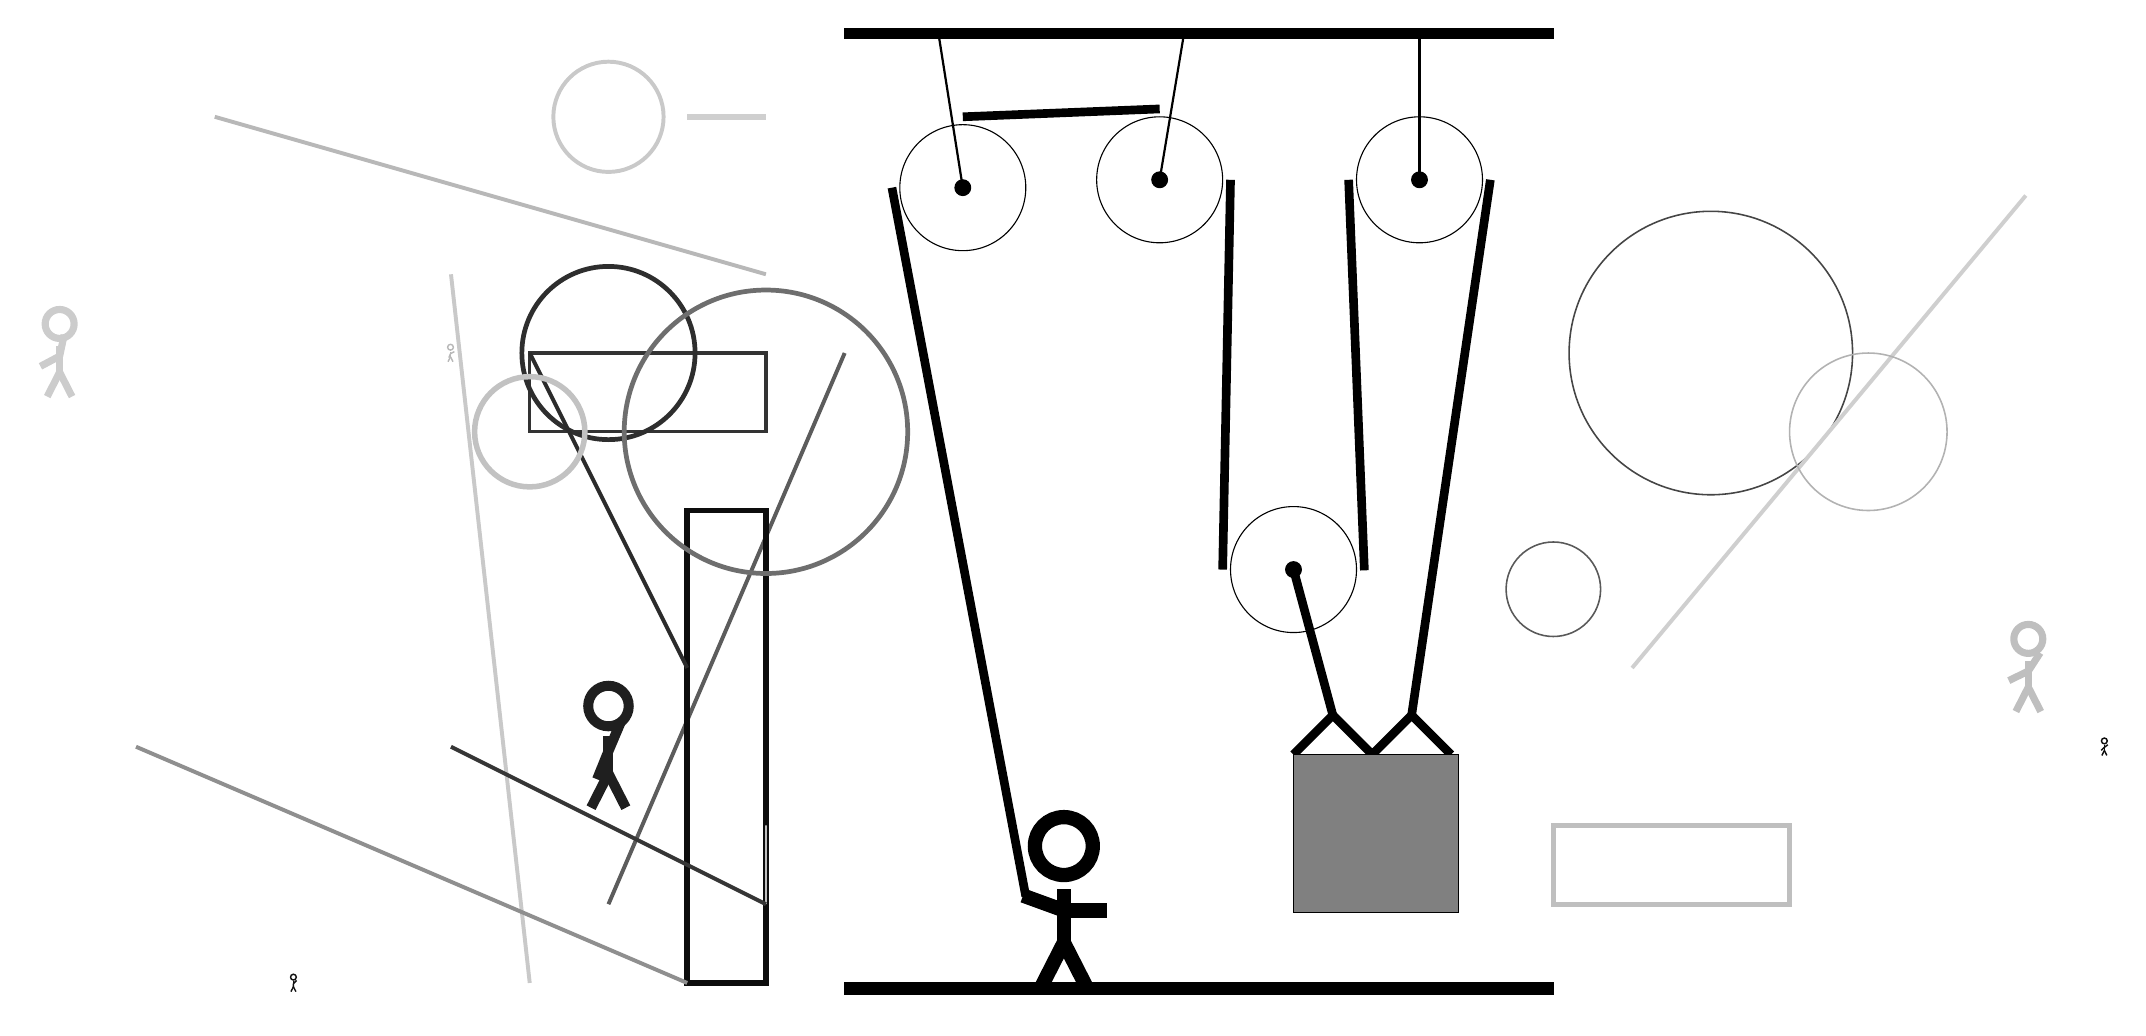
\begin{tikzpicture}
			%%%%% START %%%%%
			
			\draw[fill=black] (-3, 9) rectangle (6, 9.125);
			
			\draw (1, 7.2) circle (0.8);
			\draw[fill=black] (1, 7.2) circle (0.1);
			\draw[thick] (1, 7.2) -- (1.3, 9);
			
			\draw[line width=0.5mm, color=black!21](-8, 6) -- (-7, -3);
			
			\draw[line width=0.5mm, color=black!64](-3, 5) -- (-6, -2);
			\draw [line width=0.2mm, color=black!73](8, 5) circle (1.8);
			\draw[line width=0.7mm, color=black!95] (-4, -3) rectangle (-5, 3);
			\node[line width=0.2mm, color=black!20] at (-13, 5) {\Strichmaxerl[5][28][78]};
			
			\draw[line width=0.5mm, color=black!19](7, 1) -- (12, 7);
			\draw[line width=0.2mm, color=black!25] (-4, -1) rectangle (-4, -2);
			\draw[line width=0.7mm, color=black!19] (-4, 8) rectangle (-5, 8);
			\draw[line width=0.5mm, color=black!44](-5, -3) -- (-12, 0);
			
			\draw[line width=0.4mm, color=black!80] (-4, 5) rectangle (-7, 4);
			\draw [line width=0.2mm, color=black!30](10, 4) circle (1.0);
			\draw [line width=0.6mm, color=black!82](-6, 5) circle (1.1);
			\node[line width=0.2mm, color=black!88] at (-6, 0) {\Strichmaxerl[7][68][67]};
			
			\node[line width=0.3mm, color=black!25] at (12, 1) {\Strichmaxerl[5][26][57]};
			\draw[line width=0.5mm, color=black!79](-8, 0) -- (-4, -2);
			\node[line width=0.2mm, color=black!93] at (-10, -3) {\Strichmaxerl[1][88][45]};
			\node[line width=0.6mm, color=black!95] at (13, 0) {\Strichmaxerl[1][44][37]};
			\draw[line width=0.6mm, color=black!25] (6, -1) rectangle (9, -2);
			\draw [line width=0.2mm, color=black!65](6, 2) circle (0.6);
			\draw[line width=0.5mm, color=black!83](-5, 1) -- (-7, 5);
			\draw [line width=0.5mm, color=black!21](-6, 8) circle (0.7);
			
			\draw [line width=0.6mm, color=black!57](-4, 4) circle (1.8);
			\node[line width=0.3mm, color=black!28] at (-8, 5) {\Strichmaxerl[1][68][27]};
			\draw[line width=0.5mm, color=black!28](-4, 6) -- (-11, 8);
			\draw [line width=0.7mm, color=black!24](-7, 4) circle (0.7);
			
			
			\draw (4.3, 7.2) circle (0.8);
			\draw[fill=black] (4.3, 7.2) circle (0.1);
			\draw[thick] (4.3, 7.2) -- (4.3, 9);
			
			\draw (2.7, 2.25) circle (0.8);
			\draw[fill=black] (2.7, 2.25) circle (0.1);
			
			\draw[line width=1.1mm]  (2.7, -0.1) -- (3.2, 0.4) -- (3.7, -0.1) -- (4.2, 0.4) -- (4.7, -0.1);
			\draw[fill=black!50] (2.7, -0.1) rectangle (4.8, -2.1);
			
			\draw (-1.5, 7.1) circle (0.8);
			\draw[fill=black] (-1.5, 7.1) circle (0.1);
			\draw[thick] (-1.5, 7.1) -- (-1.8, 9);
			
			\draw[line width=1.1mm](-0.7, -1.9) --  (-2.4, 7.1);
			\centerarc[line width=1.1mm](-1.5, 7.1)(90:180:0.9);
			\draw[line width=1.1mm](-1.5, 8.0) -- (1, 8.1);
			\centerarc[line width=1.1mm](1, 7.2)(0:90:0.9);
			\draw[line width=1.1mm](1.9, 7.2) -- (1.8, 2.25);
			\centerarc[line width=1.1mm](2.7, 2.25)(180:370:0.9);
			\draw[line width=1.1mm] (3.6, 2.24) -- (3.4, 7.2);
			\centerarc[line width=1.1mm](4.3, 7.2)(0:180:0.9);
			\draw[line width=1.1mm](4.2, 0.4) -- (5.2, 7.2);
			\draw[line width=1.1mm] (3.2, 0.4) -- (2.7, 2.25);
			
			\node at (-0.2, -2) {\Strichmaxerl[10][-20][0]};
			
			\draw[fill=black] (-3, -3) rectangle (6, -3.15);
			
			%%%%% END %%%%%
		\end{tikzpicture}
	\end{figure}	
\end{document}